\documentclass[conf]{new-aiaa}
%\documentclass[journal]{new-aiaa} for journal papers
\usepackage[utf8]{inputenc}

\usepackage{graphicx}
\usepackage{amsmath}
\usepackage[version=4]{mhchem}
\usepackage{siunitx}
\usepackage{longtable,tabularx}
\usepackage{interval}
\usepackage{subcaption}
\usepackage{algorithm}
\usepackage{algpseudocode}

\setlength\LTleft{0pt} 

\title{Reinforced Tanks}

\author{Lingfeng Chen}
\author{Lingfeng Chen, Martin Fernandez de Retana, Irune Olivares, Beñat Ramirez}

\begin{document}

\maketitle

\begin{abstract}
We developed a adversarial multi-agent reinforcement learning environment to simulate tank battles. The environment is built using purely Python and we also implement several optimizations to speed up the simulation and reduce the inference cost during the training and testing phases. The objective was to create an environment that could be used to train relatively complex agents in a acceptable time using limited computational resources. Every decision over the design of the environment was made with this goal in mind. We also provide several baseline agents that can be used as a starting point for further experiment. This document describes the environment, the design decisions made and the baseline agents implemented, as well as some experiments and results obtained. The source code can be found at \href{https://github.com/Lingfeng555/ReinforcedTanks}{Github repository}
\end{abstract}

\section{Nomenclature}

{\renewcommand\arraystretch{1.0}
\noindent\begin{longtable*}{@{}l @{\quad=\quad} l@{}}
$\pi$  & policy \\
$a$ &    action \\
$s$& state \\
$t_i$ & tensor of one tank of the team side \\
$e_i$ & tensor of one tank of the enemy side \\
$b_i$ & tensor of one bullet of the enemy side \\
$W$   & map width \\
$H$ & map height \\
$\theta$ & angle of the entity \\
$D_c(t)$ & Proximity of the tank $t$ to the center of the arena \\
$R(s)$ & Reward function at state $s$ \\
$c$ & center of the arena ($W$/2, $H$/2) \\
\end{longtable*}}

\section{Introduction}

\subsection{Context and motivation}

The development of this project was motivated by the organization of a tournament in which participants (students at the University of Deusto) would develop agents to compete in a tank battle environment, which also give this an educational purpose, which means that the final solution should be friendly for the students. The main goal was to create an environment that could be used to train relatively complex agents in a acceptable time using limited computational resources. Every decision over the design of the environment was made with this goal in mind. As reference we took the laptop offered by the University of Deusto as reference with a i5-13500U processor and 16GB of RAM  with no GPU available. As well as the developement of this project also fits in the criteria of the Reinforcement Learning subject, so it was also motivated by the need of a final project for this subject.

The tournament is essentially a model search over the space of possible agents that can be developed for this environment and the designed reward function which will relied heavily on the capacity of the agents to learn good strategies to defeat the opponent. The participants will be provided with several baseline agents that can be used as a starting point for further experiment. They will design their reward functions and train their agents using the provided environment. Finally, the trained agents will compete against each other in a series of matches to determine the winner of the tournament.

No matter the reward function the environment dictates the rules of the game and the possible actions and observations that the agents can take. But different strategies can emerge depending on the reward function used during training. In this document we provide an example of a reward function that describes a very basic strategy that can be used as a starting point for further experiment.

\subsection{Objectives and scope}

The objective of the game is a competitive battle between two teams of tanks, where each team aims to destroy the opponent’s tanks. The main rules and mechanics of the game are as follows:

\begin{itemize}
    
    \item Each team consists of two tanks, and each match has a maximum duration of 4000 time steps.
    
    \item A team wins the match if it destroys all opponent tanks before the time limit is reached.
    
    \item If neither team destroys all opponent tanks, the winner is determined by the number of tanks remaining alive at the end of the match.
    
    \item In case of a tie in the number of remaining tanks, the team whose team center, defined as the average position of all their alive tanks, is nearest to the center of the arena is declared the winner.
    
    \item Each tank is able to shoot projectiles that destroy opponent tanks upon direct impact.
    
    \item Projectiles can bounce off arena walls, with a maximum of three bounces before disappearing.
    
    \item Each tank is limited to having only one projectile in the air at any given time and cannot shoot again until the current projectile disappears.
    
    \item Tanks can move freely within the arena and may collide with walls or other tanks during gameplay.
\end{itemize}

\begin{figure}[h!]
    \centering
    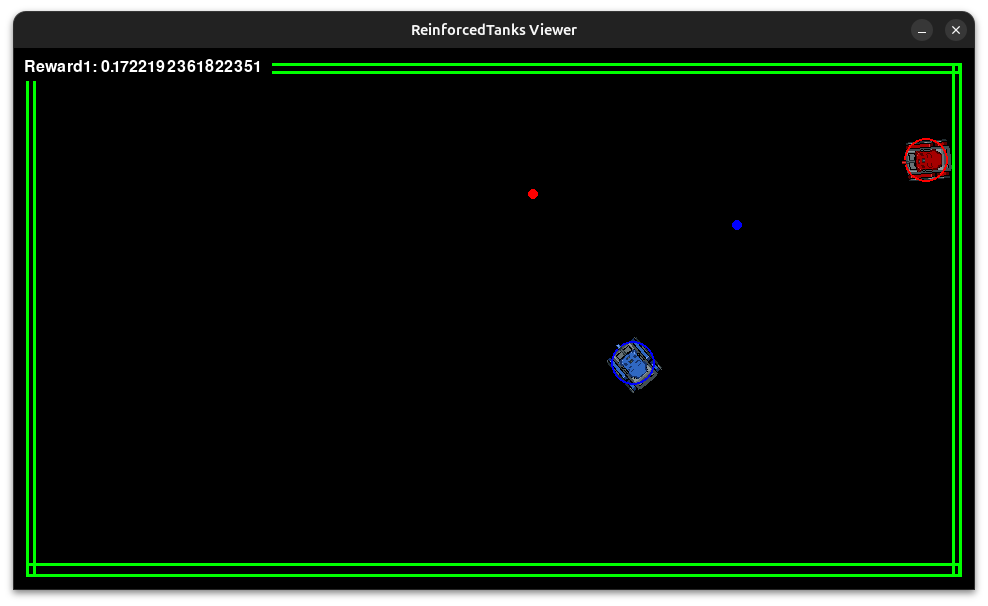
\includegraphics[width=0.5\textwidth]{images/tank_match.png}
    \caption{Tank Battle Environment Overview}
    \label{fig:tank_battle}
\end{figure}

Due to the referenced hardware limitations the main objective when designing the environment was to keep the computational cost as low as possible. This meant that the simulation had to be kept as simple as possible while still providing a challenging environment for the agents to learn and compete in. This meant that the number of agents, the complexity of the observation and action spaces and the complexity of the physics simulation had to be kept to a minimum. We provide the option of parallelizing the simulation to further reduce the training time, but this is not a requirement, as the environment can be used in a single thread. Originally there were 3 tanks per team, and more inside walls but this increase the observation space and the computational cost of the simulation too much, therefore we reduced the number of tanks to 2 per team and removed the inner walls. We also experiment several different train loops and agent architectures to further reduce the training time, and priotizing the exploration of the environment over the complexity of the agent. Check on Figure \ref{fig:tank_battle}.

\section{Environment}

\subsection{Observation space}

Several design decisions were made in the definition of the observation space $s$ with the objective of providing sufficient information for the agents to learn effective strategies while maintaining a compact state representation, thereby reducing the computational cost of both simulation and training. The observation space $s$ is defined as an array composed of two pairs of matrices, corresponding to the controlled (red) team and the opponent (blue) team reflecting all the enviroment overservable, making the agent omniscient. Thus, the complete state representation is given by:
\[
s = \{(T, B_t), (E, B_e)\}.
\]

The matrix $T = \{t_0, t_1\}$ represents the states of the tanks belonging to the controlled team, while $E = \{e_0, e_1\}$ represents the states of the enemy tanks. Similarly, the matrices $B_t = \{b_{t_0}, b_{t_1}\}$ and $B_e = \{b_{e_0}, b_{e_1}\}$ encode the states of the bullets fired by the controlled and enemy teams, respectively.

Each matrix is organized such that each row corresponds to a single entity. The state of a tank is defined as
\[
t_i = \left[\text{alive} \in \{0,1\},\ \theta \in \interval[open right]{0}{360},\ x \in \interval{0}{W},\ y \in \interval{0}{H}\right],
\]
where \textit{alive} indicates whether the tank is active, $\theta$ denotes its orientation in degrees, and $(x,y)$ represents its position within an arena of width $W$ and height $H$. The same representation is used for enemy tanks $e$.

The state of a bullet is defined as
\[
b_i = \left[\text{alive} \in \{0,1\},\ \theta \in \interval[open right]{0}{360},\ c \in \interval{0}{3},\ x \in \interval{0}{W},\ y \in \interval{0}{H}\right],
\]
where $c$ denotes the number of wall bounces performed by the projectile, capped at a maximum of three.

If the policy is playing for the blue team, then all the observation will be mirrored so the model can be reused as enemy model.

\subsection{Action space}

The action space $a$ is defined as a discrete vector composed of movement, rotation, and shooting commands:
\[
a = \{\text{move} \in \{0,1\}^3,\ \text{rotate} \in \{0,1\}^3,\ \text{shoot} \in \{0,1\}^2\}.
\]

The agent would move according to the following rules:

\begin{itemize}
    \item \textbf{Movement commands:}
    \begin{itemize}
        \item 0: Stay still
        \item 1: Move forward
        \item 2: Move backward
    \end{itemize}

    \item \textbf{Rotation commands:}
    \begin{itemize}
        \item 0: No rotation
        \item 1: Rotate left
        \item 2: Rotate right
    \end{itemize}

    \item \textbf{Shooting commands:}
    \begin{itemize}
        \item 0: Do not shoot
        \item 1: Shoot
    \end{itemize}
\end{itemize}


This action space is adapted to the training loop that will be explained later to reduce the complexity of the agent and speed up the training process. The movement commands allow tanks to move forward, backward, or remain stationary, but only one tank can be controlled at a step. 

\subsection{Reward structure}

The reward function was designed to encourage the agent to maintain an advantage over the opponent by (i) maximizing the number of tanks remaining alive and (ii) prioritizing central positioning as a tie-break criterion. The reward is defined as
\[
R(s)=
\begin{cases}
\displaystyle +100,
& \text{if } \sum_{i=0}^{1} \text{alive}(e_i) = 0, \\[6pt]

\displaystyle -100,
& \text{if } \sum_{i=0}^{1} \text{alive}(t_i) = 0, \\[6pt]

\displaystyle \sum_{i=0}^{1} \text{alive}(t_i) - \sum_{i=0}^{1} \text{alive}(e_i),
& \text{if } \sum_{i=0}^{1} \text{alive}(t_i) \neq \sum_{i=0}^{1} \text{alive}(e_i), \\[8pt]

\displaystyle D_c(t^i) - D_c(e^\star),
& \text{otherwise},
\end{cases}
\]
where $t^i$ denotes the tank currently controlled by the agent, and $e^\star$ denotes the closest \emph{alive} enemy tank to the center of the arena, defined as
\[
e^\star = \arg\min_{e_i:\,\text{alive}(e_i)=1} d(e_i,c),
\]
with $d(\cdot,\cdot)$ denoting the Euclidean distance and $c=(W/2,H/2)$ the arena center. The center-proximity term is defined as
\[
D_c(u)=\left(1-\frac{d(u,c)}{d_{\max}}\right)^k,
\qquad
d_{\max}=\sqrt{(W/2)^2+(H/2)^2},
\]
where $k$ is a hyperparameter controlling the importance of central positioning.

Undesired behaviors, such as camping near the center of the arena without actively engaging the opponent, may emerge as a consequence of the proposed reward formulation. However, given the objective of this environment, rather than explicitly preventing such behaviors at the environment level, they are deliberately permitted and leveraged as an evaluation mechanism. Specifically, the emergence of these behaviors serves to assess how rapidly and effectively the proposed architecture adapts to and exploits the reward structure. This design choice also preserves flexibility, allowing users to define and experiment with more sophisticated reward functions that explicitly discourage such strategies if desired. Check on Figure \ref{fig:reward_exploit}. On the other hand, this may be the intention of the user, therefore we leave this decision to the user.

\begin{figure}[t]
    \centering
    \begin{subfigure}[t]{0.48\textwidth}
        \centering
        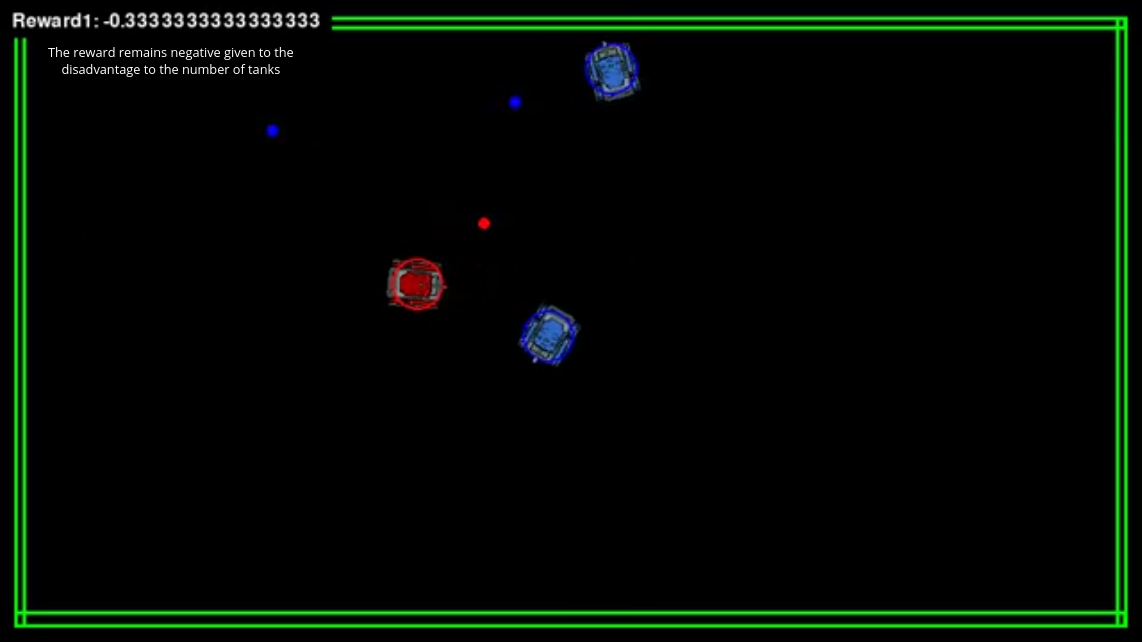
\includegraphics[width=\textwidth]{images/Reward_Exploit_Before.png}
        \caption{The reward remains negative due to the disadvantage in the number of tanks.}
        \label{fig:reward_exploit_before}
    \end{subfigure}\hfill
    \begin{subfigure}[t]{0.48\textwidth}
        \centering
        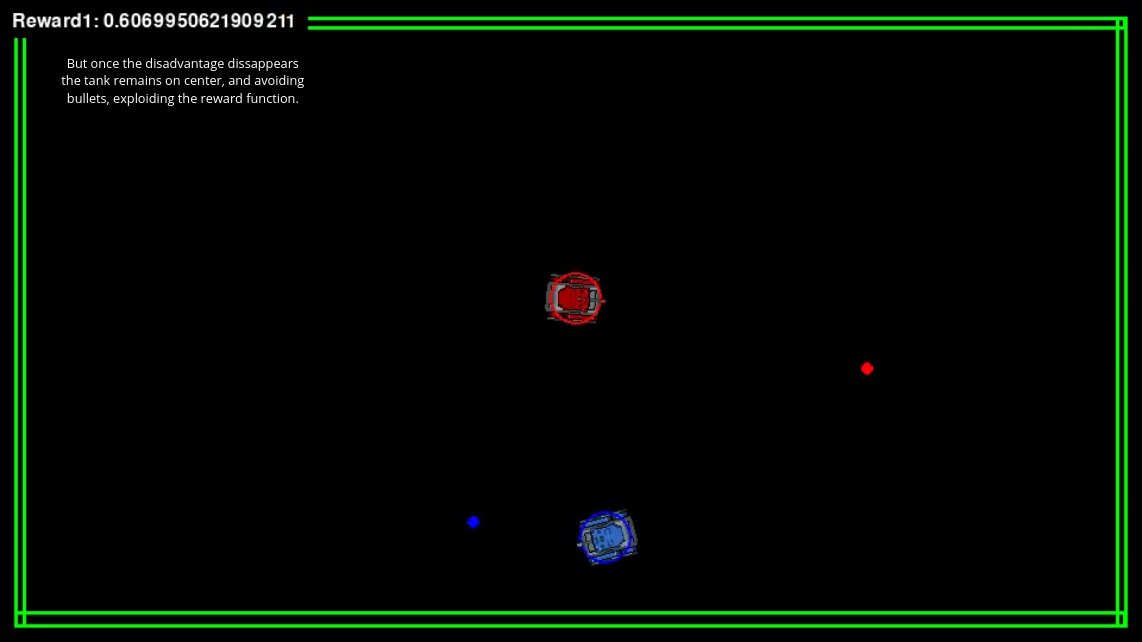
\includegraphics[width=\textwidth]{images/Reward_Exploit_After.png}
        \caption{Once the disadvantage disappears, the tank remains near the center and avoids bullets, thereby exploiting the reward function.}
        \label{fig:reward_exploit_after}
    \end{subfigure}
    \caption{Illustration of reward exploitation by camping near the arena center. \href{https://youtu.be/jMT5M7QSV5M}{Watch the complete video}}
    \label{fig:reward_exploit}
\end{figure}

\section{Agent and Training loop}

\subsection{Agent}
Given that the state $s$ fully represents the environment and that the arena walls remain unchanged across different matches, the environment satisfies the Markov property. Therefore, we designed the agent architecture without any explicit memory mechanism, as the optimal policy can be expressed as a function of the current state alone.

Given to the requirement of the project to be able to train relatively complex agents in a acceptable time using limited computational resources, the agent architecture was designed to be as simple as possible while still being able to learn effective strategies. The agent is implemented using a PPO algorithm \cite{PPO} with a custom feature extractor that processes the observation space and outputs a compact representation that can be used by the policy network. The complete agent has around 53K parameters, which is relatively small and trainable in CPU only. We also implemented several considerations in the design of the feature extractor with mechanics of the game in mind. Which means that this is a model-based approach.

\subsection{Training Loop}
%Seguro que esto lo ha hecho alguien mas, hay que buscarlo y citarlo%
The training loop is designed to optimize the learning process by alternating control between the two tanks of the controlled team. At each time step, only one tank is actively controlled by the agent and receives the corresponding observation and reward.

For the team tanks in state $s$, we swap the position of the currently controlled tank to the first position in the state tensor, ensuring that the agent always controls the first tank $t_0$ in the tensor representation. This design choice simplifies the action space and reduces the complexity of the agent, as the policy only needs to learn to control a single tank at a time while implicitly considering the state of the remaining tanks. Once all tanks in $T$ have received their corresponding actions and rewards at step $s_i$, the actions for the enemy team $E$ are also computed and executed at the same step $s_i$.

Also the shoot action is only available to the currently controlled tank if it does not have an active bullet in the arena. Which means that all the updates related to the policy head for the shoot action are only done when the currently controlled tank is able to shoot. Regarding the movement and rotation actions, they are always available to the currently controlled tank. This reduces the complexity of the action space and enables more focused learning for the agent.

With this design, the policy effectively learns to control only one agent at a time while still being aware of the overall team state. This approach reduces the dimensionality of the action space and enables more focused learning, leading to faster convergence and improved performance, while remaining effective in a multi-agent environment.

\subsection{Design decisions}

The feature extractor is composed of two functions that operate on the current state of the environment, $T_T$ and $T_B$. Notably, angular features are represented using a polar-like encoding, decomposed into sine and cosine components, in order to avoid discontinuities in the angular space. For instance, angles of $5^\circ$ and $355^\circ$ are very close in physical space but would appear distant under a linear representation. In addition, other informative features, such as the distance between entities and the distance to the center of the arena, are also included to provide richer contextual information to the model, as these quantities are explicitly considered in the game rules.

The functions $T_T$ and $T_B$ are responsible for extracting relational embeddings from tank--tank and tank--bullet interactions, respectively. These embeddings capture the spatial and angular relationships between the main tank and other entities in the environment, providing a rich and informative representation of the current state.

\subsubsection{Tank-Tank interactions}
Let $t_0$ denote the main tank features and $t$ another tank features, and $\mathcal{T}$ be any set of tanks $T$ or $E$. The module $f(t_0,t)$ builds a relational embedding by extracting and combining the following components:

\begin{itemize}
    \item {Positions, representing the spatial coordinates of the main tank and the other tank, respectively:}
    \[
    \mathbf{p}_0 = t_0[-2:], \qquad \mathbf{p} = t[-2:], \qquad \mathbf{p}_0,\mathbf{p}\in\mathbb{R}^2,
    \]

    \item {Inter-tank distance, encoding the euclidean distance between both tanks:}
    \[
    d = \left\lVert \mathbf{p}_0 - \mathbf{p} \right\rVert_2,
    \]

    \item {Relative distance to arena center, which captures whether the main tank is closer to or farther from the center than the other tank:}
    Let $\mathbf{c}\in\mathbb{R}^2$ denote the arena center. We define
    \[
    d_c = \left\lVert \mathbf{p}_0 - \mathbf{c} \right\rVert_2 - \left\lVert \mathbf{p} - \mathbf{c} \right\rVert_2,
    \]

    \item {Tank orientations, where angles are given in degrees and converted to radians as:}
    \[
    \theta_0 = t_0[1], \qquad \theta = t[1], \qquad
    \theta_0^{(r)}=\frac{\pi}{180}\,\theta_0,
    \qquad
    \theta^{(r)}=\frac{\pi}{180}\,\theta.
    \]

    \item {Wrapped angular difference, representing the signed relative orientation between both tanks, invariant to angle wrapping:}
    \[
    \Delta\theta
    =
    \frac{\pi}{180}\left(\left(\left|\theta_0-\theta+180\right|\bmod 360\right)-180\right),
    \]

    \item {Trigonometric orientation encoding, which provides a continuous representation of angular information:}
    \[
    \mathbf{x}_{c}
    =
    [\cos\theta_0^{(r)};\cos\theta^{(r)};\sin\theta_0^{(r)};\sin\theta^{(r)}],
    \]
\end{itemize}

All components are concatenated into a single feature vector
\[
\mathbf{x}
=
[\mathbf{p}_0;\mathbf{p};d;d_c;\mathbf{x}_{c};\Delta\theta],
\]
which is passed through a learned projection network $p_{\theta}$ to obtain the final relational embedding:
\[
f(t_0, t) = p_{\theta}(\mathbf{x}) \in \mathbb{R}^{d_{tt}}.
\]
If tank $t$ is not alive, the function $f(t_0, t)$ returns an empty embedding, thereby avoiding unnecessary computation.

The tank--tank module $T_T$ is defined as the application of $f$ to each tank $t$ in the set of tanks $\mathcal{T}$:
\[
T_T(t_0, \mathcal{T}) =
\left\{\, f(t_0, t) \;\middle|\; t \in \mathcal{T},\; t \text{ is alive} \,\right\}.
\]

\subsubsection{Tank-Bullet interactions}
Let $t_0$ denote the main tank features and $b$ a bullet feature vector, and let $\mathcal{B}$ be the set of bullets present in the environment. The module $g(t_0,b)$ builds a relational embedding by extracting and combining the following components:

\begin{itemize}
    \item {Positions, representing the spatial coordinates of the main tank and the bullet, respectively:}
    \[
    \mathbf{p}_0 = t_0[-2:], \qquad \mathbf{p}_b = b[-2:], \qquad \mathbf{p}_0,\mathbf{p}_b\in\mathbb{R}^2,
    \]

    \item {Tank and bullet orientations, where angles are given in degrees and converted to radians as:}
    \[
    \theta_0 = t_0[-3], 
    \qquad 
    \theta_b = b[-4],
    \qquad
    \theta_0^{(r)}=\frac{\pi}{180}\,\theta_0,
    \qquad
    \theta_b^{(r)}=\frac{\pi}{180}\,\theta_b.
    \]

    \item {Bullet--tank distance, encoding the Euclidean distance between the bullet and the main tank:}
    \[
    d = \left\lVert \mathbf{p}_b - \mathbf{p}_0 \right\rVert_2,
    \]

    \item {Bullet trajectory distance, measuring the perpendicular distance from the main tank to the bullet trajectory:}
    Let $\mathbf{p}_0=(x_0,y_0)$ and $\mathbf{p}_b=(x_b,y_b)$. Defining the bullet trajectory slope
    \[
    m_b = \tan(\theta_b^{(r)}),
    \qquad
    n_b = y_b - m_b x_b,
    \]
    the distance is given by
    \[
    d_{\text{traj}}
    =
    \frac{\left|m_b x_0 - y_0 + n_b\right|}{\sqrt{m_b^2 + 1}}.
    \]

    \item {Trigonometric orientation encoding, which provides a continuous representation of angular information:}
    \[
    \mathbf{x}_{c}
    =
    [\cos\theta_0^{(r)};\cos\theta_b^{(r)};\sin\theta_0^{(r)};\sin\theta_b^{(r)}].
    \]
\end{itemize}

All components are concatenated into a single feature vector
\[
\mathbf{x}
=
[d;\,d_{\text{traj}};\,\mathbf{p}_0;\,\mathbf{p}_b;\,\mathbf{x}_{c}],
\]
which is passed through a learned projection network $p_{\theta}$ to obtain the final relational embedding:
\[
g(t_0, b) = p_{\theta}(\mathbf{x}) \in \mathbb{R}^{d_{tb}}.
\]

The tank--bullet module $T_B$ is defined as the application of $g$ to each bullet $b$ in the set of bullets $\mathcal{B}$:
\[
T_B(t_0, \mathcal{B}) =
\left\{\, g(t_0, b) \;\middle|\; b \in \mathcal{B} \,\right\}.
\]

\subsubsection{Feature extractor}
After computing the aggregated embeddings for each relational component, namely bullets, allied tanks, and enemy tanks, the feature extractor concatenates them along the feature dimension to form a single fixed-size representation. Let
$\bar{\mathbf{z}}_{B}\in\mathbb{R}^{d_{tb}}$,
$\bar{\mathbf{z}}_{T}\in\mathbb{R}^{d_{tt}}$, and
$\bar{\mathbf{z}}_{E}\in\mathbb{R}^{d_{tt}}$
denote the aggregated embeddings produced by the bullet module, the allied tank module, and the enemy tank module, respectively. The final input embedding is then
\[
\mathbf{h} = [\bar{\mathbf{z}}_{B};\bar{\mathbf{z}}_{T};\bar{\mathbf{z}}_{E}],
\]
which is passed through a final projection network $p_f$  to obtain the output of the feature extractor:
\[
\mathbf{z} = q_{\phi}(\mathbf{h}).
\]

\subsection{Training procedure}

We adopt a league-based self-play training strategy \cite{NASHSelfPlaying}. At the beginning of each match, the environment is reset and the tanks of both teams are initialized at random positions and orientations within predefined spawn zones. For each episode, the environment randomly selects a model from the current league to act as the policy for the blue team. If no opponent model is available, the blue team follows a static policy and remains idle.

A match terminates when either one team destroys all opponent tanks or a predefined time limit is reached. At each simulation step, only one tank per team is controlled by its corresponding policy; control alternates between the two tanks of each team at successive steps. The same mechanism is applied symmetrically to both the red and blue teams, each using its own policy.

During a match, all interactions are recorded and stored in a rollout buffer. Once the episode concludes, the collected experience is used to update the red team policy using the Proximal Policy Optimization (PPO) \cite{PPO} algorithm. This process is repeated until the total number of training timesteps specified by the user is reached. The model is periodically saved according to a user-defined interval, progressively building a pool of opponent policies for self-play.

In addition, a curriculum learning \cite{CVLEARNING} strategy is employed. At a high level, the user may define multiple reward functions and specify the number of epochs allocated to each, enabling a manually designed curriculum. Beyond this explicit setup, an implicit curriculum is always active through the progressive expansion of spawn zones. During training, the model is updated at least three times per epoch, and at each update the allowed spawn regions are expanded. Initially, tanks spawn near the center of the arena; in later stages, they may spawn at any valid position on their respective side of the map. This gradual increase in initial-state complexity encourages the agent to first learn simple survival and positioning behaviors, and later develop more advanced strategic and tactical decision-making. The complete training procedure is summarized in Algorithm \ref{alg:league_selfplay_curriculum}.

\begin{algorithm}[t]
\caption{League-based self-play training with curriculum over reward functions and spawn stages}
\label{alg:league_selfplay_curriculum}
\begin{algorithmic}[1]
\Require Learning schedule $\mathcal{S}=\{(E_i, r_i)\}_{i=1}^{N}$, timesteps per update $K$, visualization stride $s_v$, checkpoint stride $s_c$
\Require Red policy $\pi_{\text{red}}$ (trainable), league $\mathcal{L}$ (pool of opponent policies), environment $\mathcal{E}$
\Ensure Updated policy $\pi_{\text{red}}$ and updated league $\mathcal{L}$

\For{\textbf{each} $(E, r)$ \textbf{in} $\mathcal{S}$} \Comment{User-defined curriculum over reward functions}
    \State $\mathcal{E} \leftarrow \textsc{SetRewardFunction}(\mathcal{E}, r)$
    \For{$s \gets 0$ \textbf{to} $2$} \Comment{Implicit curriculum over spawn zones (3 stages)}
        \State $\mathcal{E} \leftarrow \textsc{SetStage}(\mathcal{E}, s)$
        \For{$e \gets 0$ \textbf{to} $E-1$}
            \State $v \gets (e \bmod s_v = 0)$ \Comment{Visualization flag}
            \State $c \gets (e \bmod s_c = 0)$ \Comment{Checkpoint flag}

            \Comment{On-policy data collection via league-based self-play}
            \State $\pi_{\text{blue}} \gets 
            \begin{cases}
                \textsc{SampleUniform}(\mathcal{L}), & |\mathcal{L}|>0\\
                \pi_{\text{idle}}, & \text{otherwise}
            \end{cases}$
            \State $\tau \gets \textsc{CollectRollout}(\mathcal{E}, \pi_{\text{red}}, \pi_{\text{blue}}, K)$

            \Comment{PPO update at the end of the match/rollout}
            \State $\pi_{\text{red}} \gets \textsc{PPOUpdate}(\pi_{\text{red}}, \tau)$

            \If{$c$}
                \State $\textsc{Save}(\pi_{\text{red}})$
                \State $\mathcal{L} \gets \mathcal{L} \cup \{\pi_{\text{red}}\}$ \Comment{Add to opponent pool}
            \EndIf
            \If{$v$}
                \State $\textsc{Visualize}(\pi_{\text{red}}, \pi_{\text{blue}}, \mathcal{E})$
            \EndIf
        \EndFor
    \EndFor
\EndFor
\end{algorithmic}
\end{algorithm}

\subsection{Experiments and Results}
Based on the 19 Models we provide we had the following results in during the training process, the best model achieved a win rate of 63\% against all the other models provided. The training was done using 8 parallel environments in a laptop with an i5-13500U processor and 16GB of RAM with no GPU available. The total training time was around 6 hours for 100000 timesteps per enviroment. All the results were recorded via WandB.

\begin{figure}[t]
    \centering

    \begin{subfigure}[t]{0.48\textwidth}
        \centering
        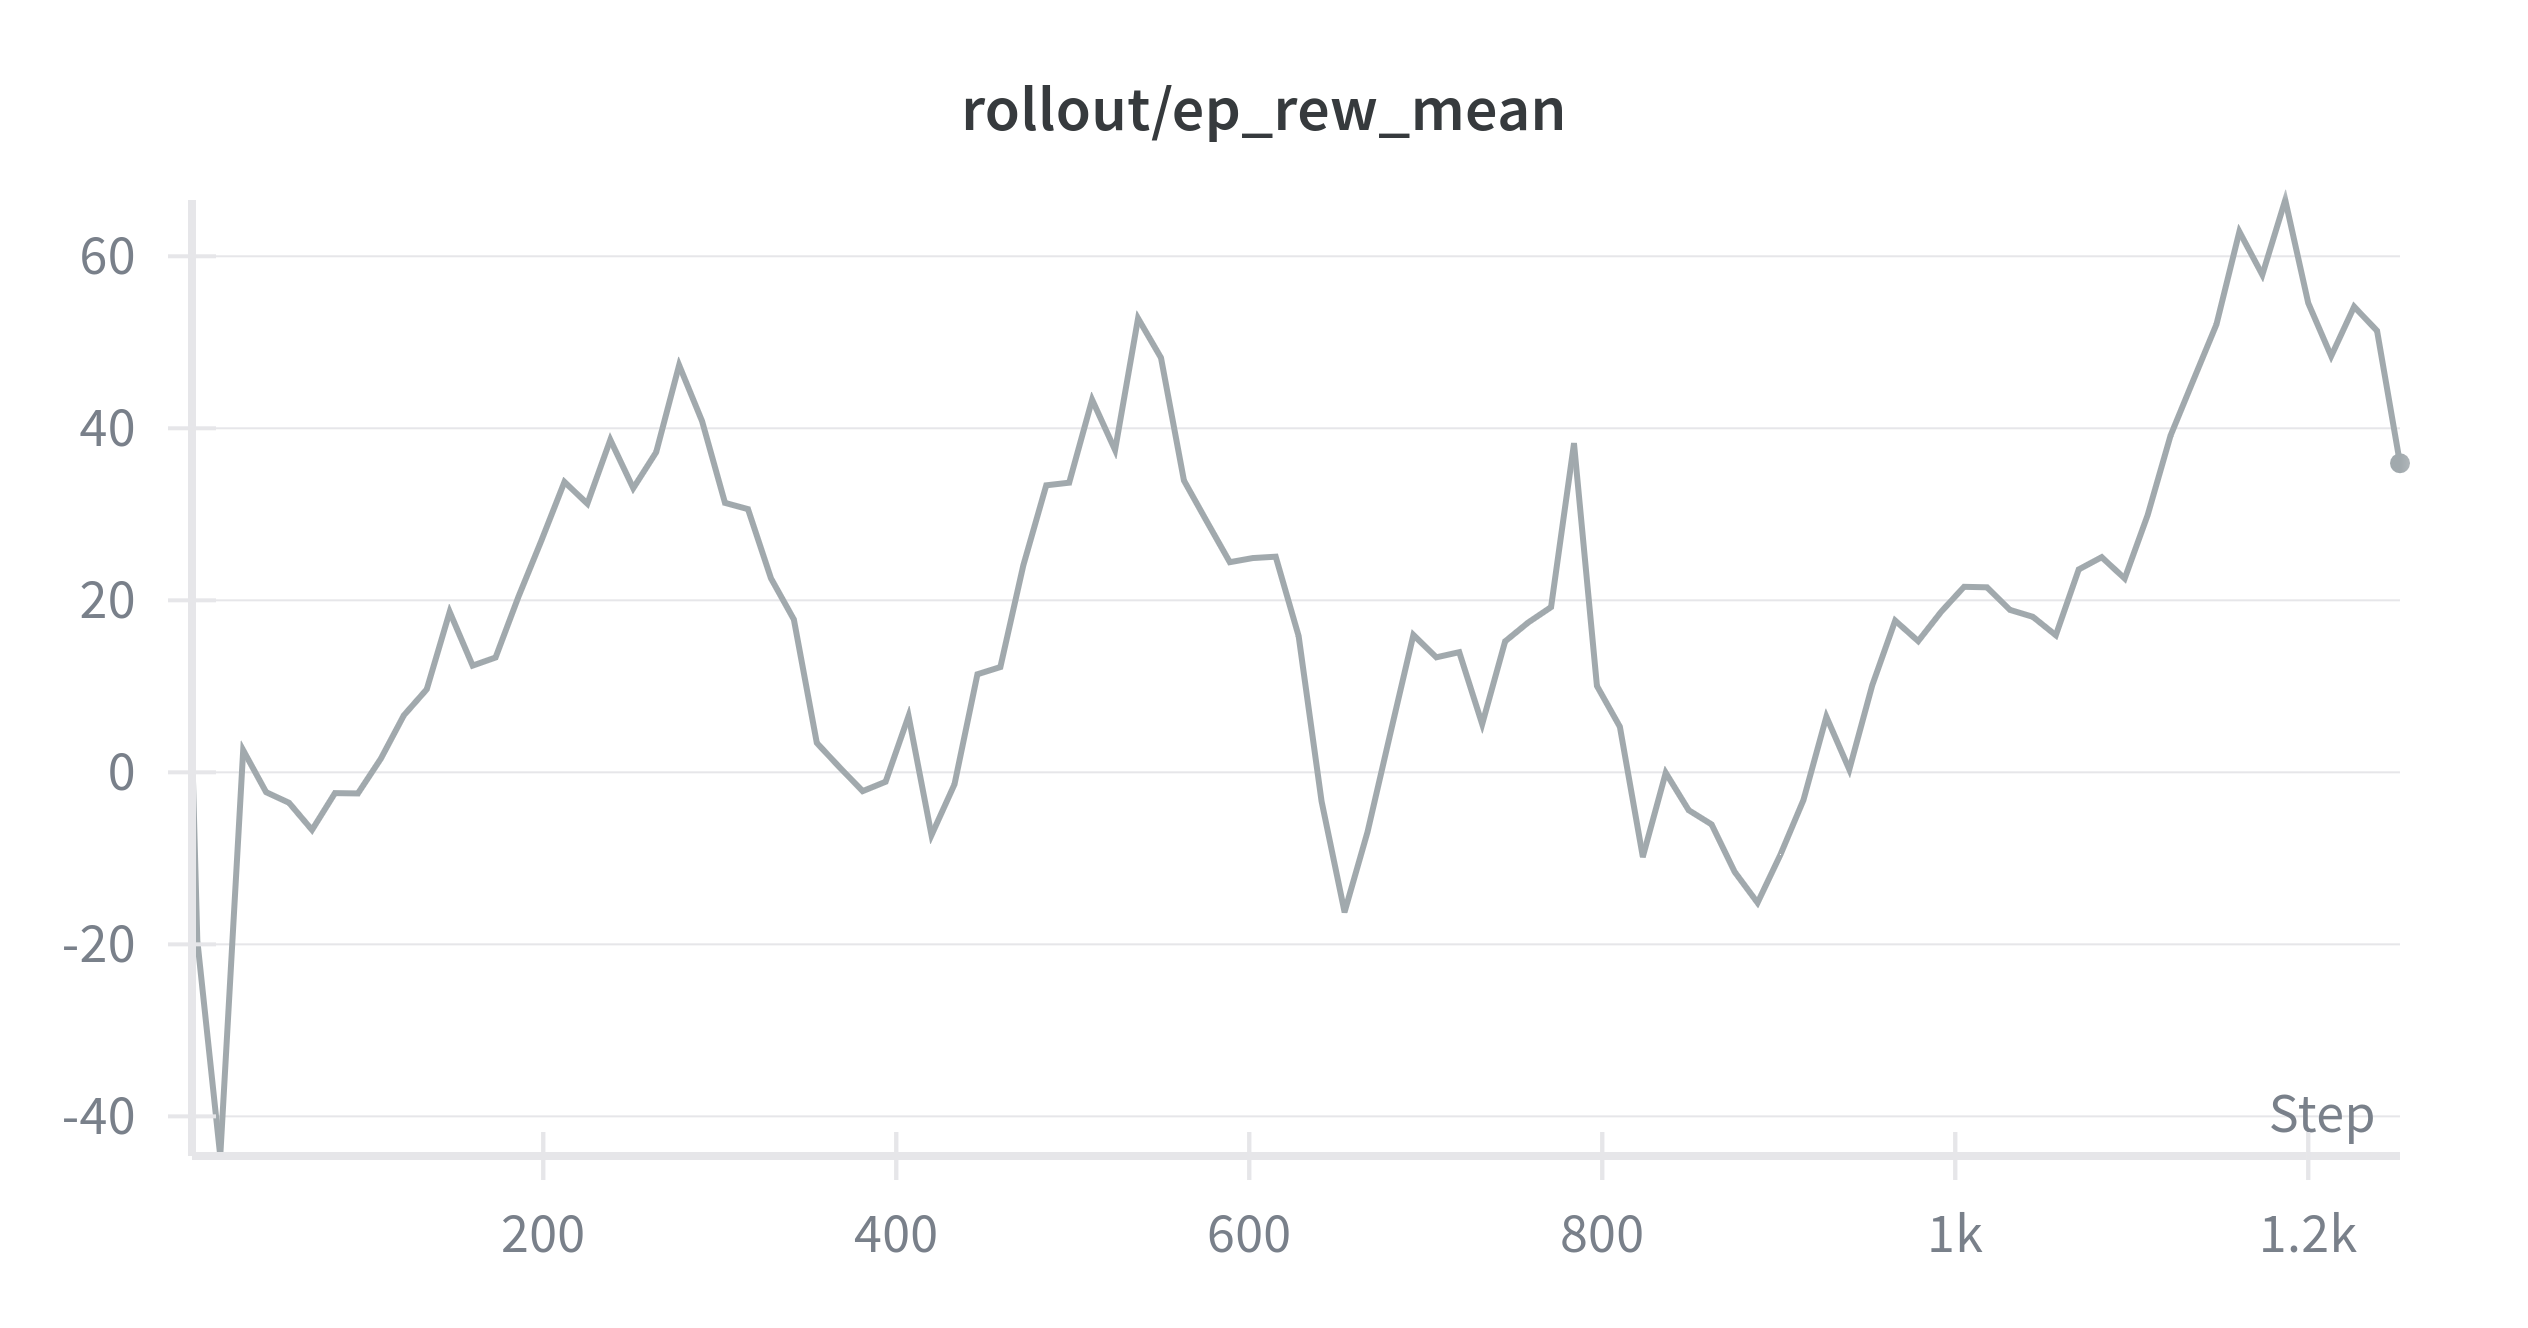
\includegraphics[width=\textwidth]{images/Reward Evolution.png}
        \caption{Reward evolution}
        \label{fig:reward_evolution}
    \end{subfigure}\hfill
    \begin{subfigure}[t]{0.48\textwidth}
        \centering
        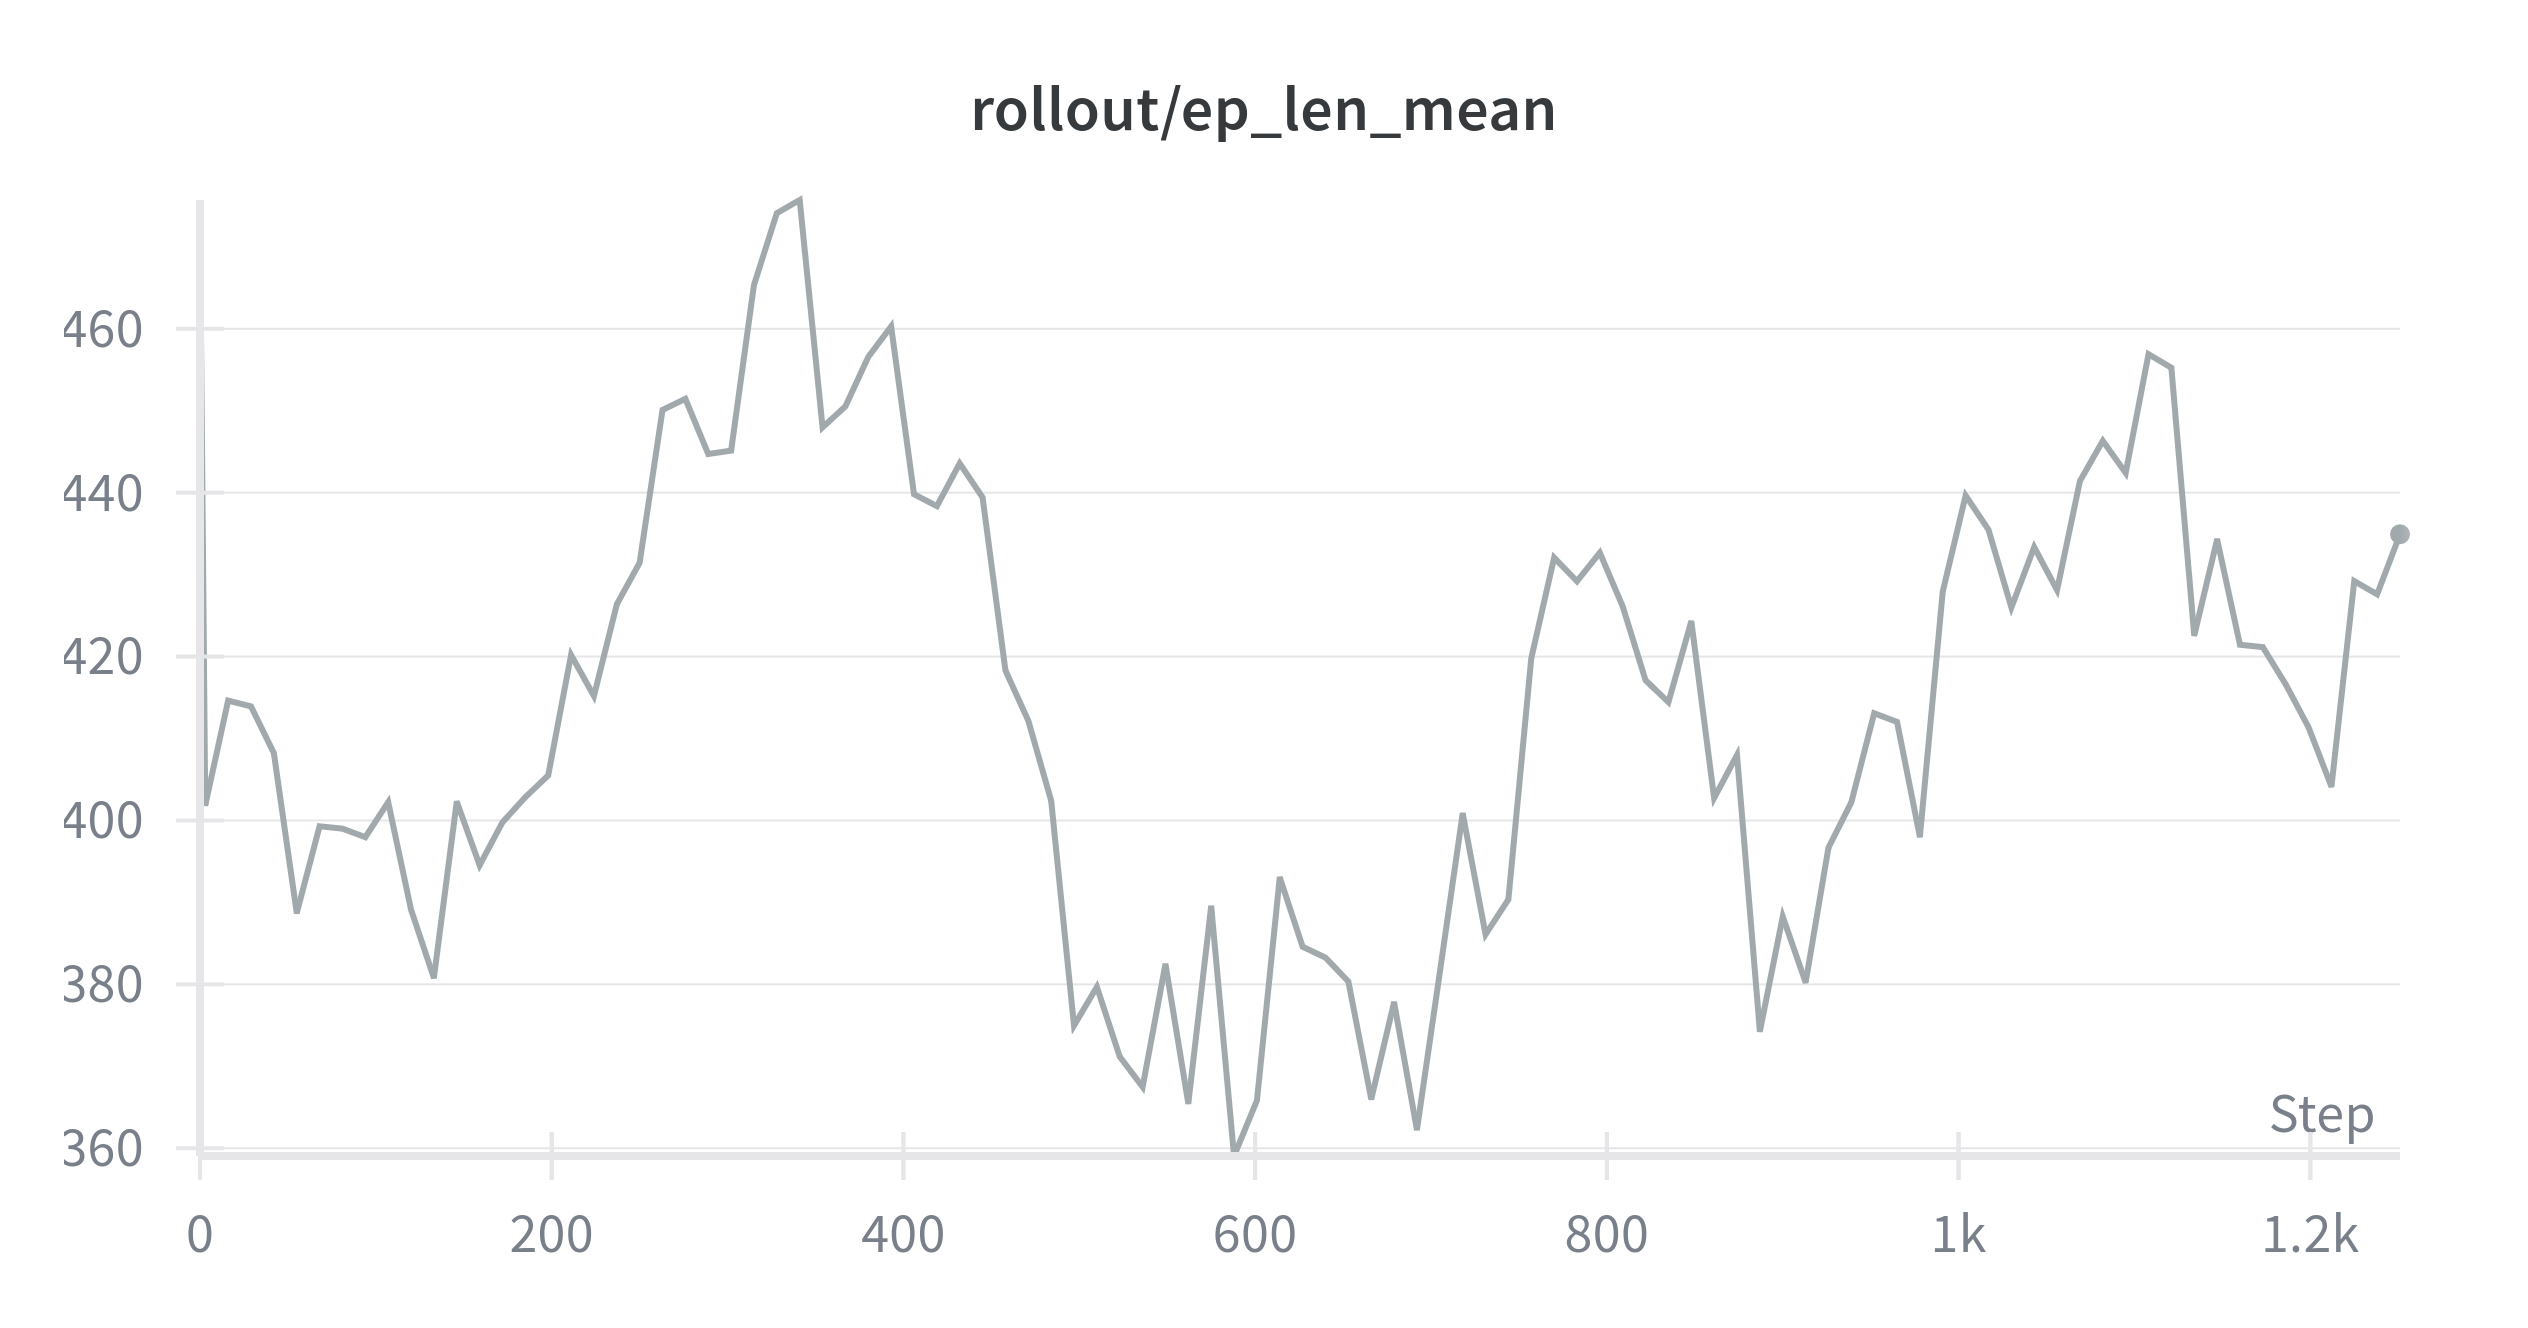
\includegraphics[width=\textwidth]{images/mean_atch_length.png}
        \caption{Mean match length}
        \label{fig:mean_match_length}
    \end{subfigure}

    \vspace{0.5em}

    \begin{subfigure}[t]{0.48\textwidth}
        \centering
        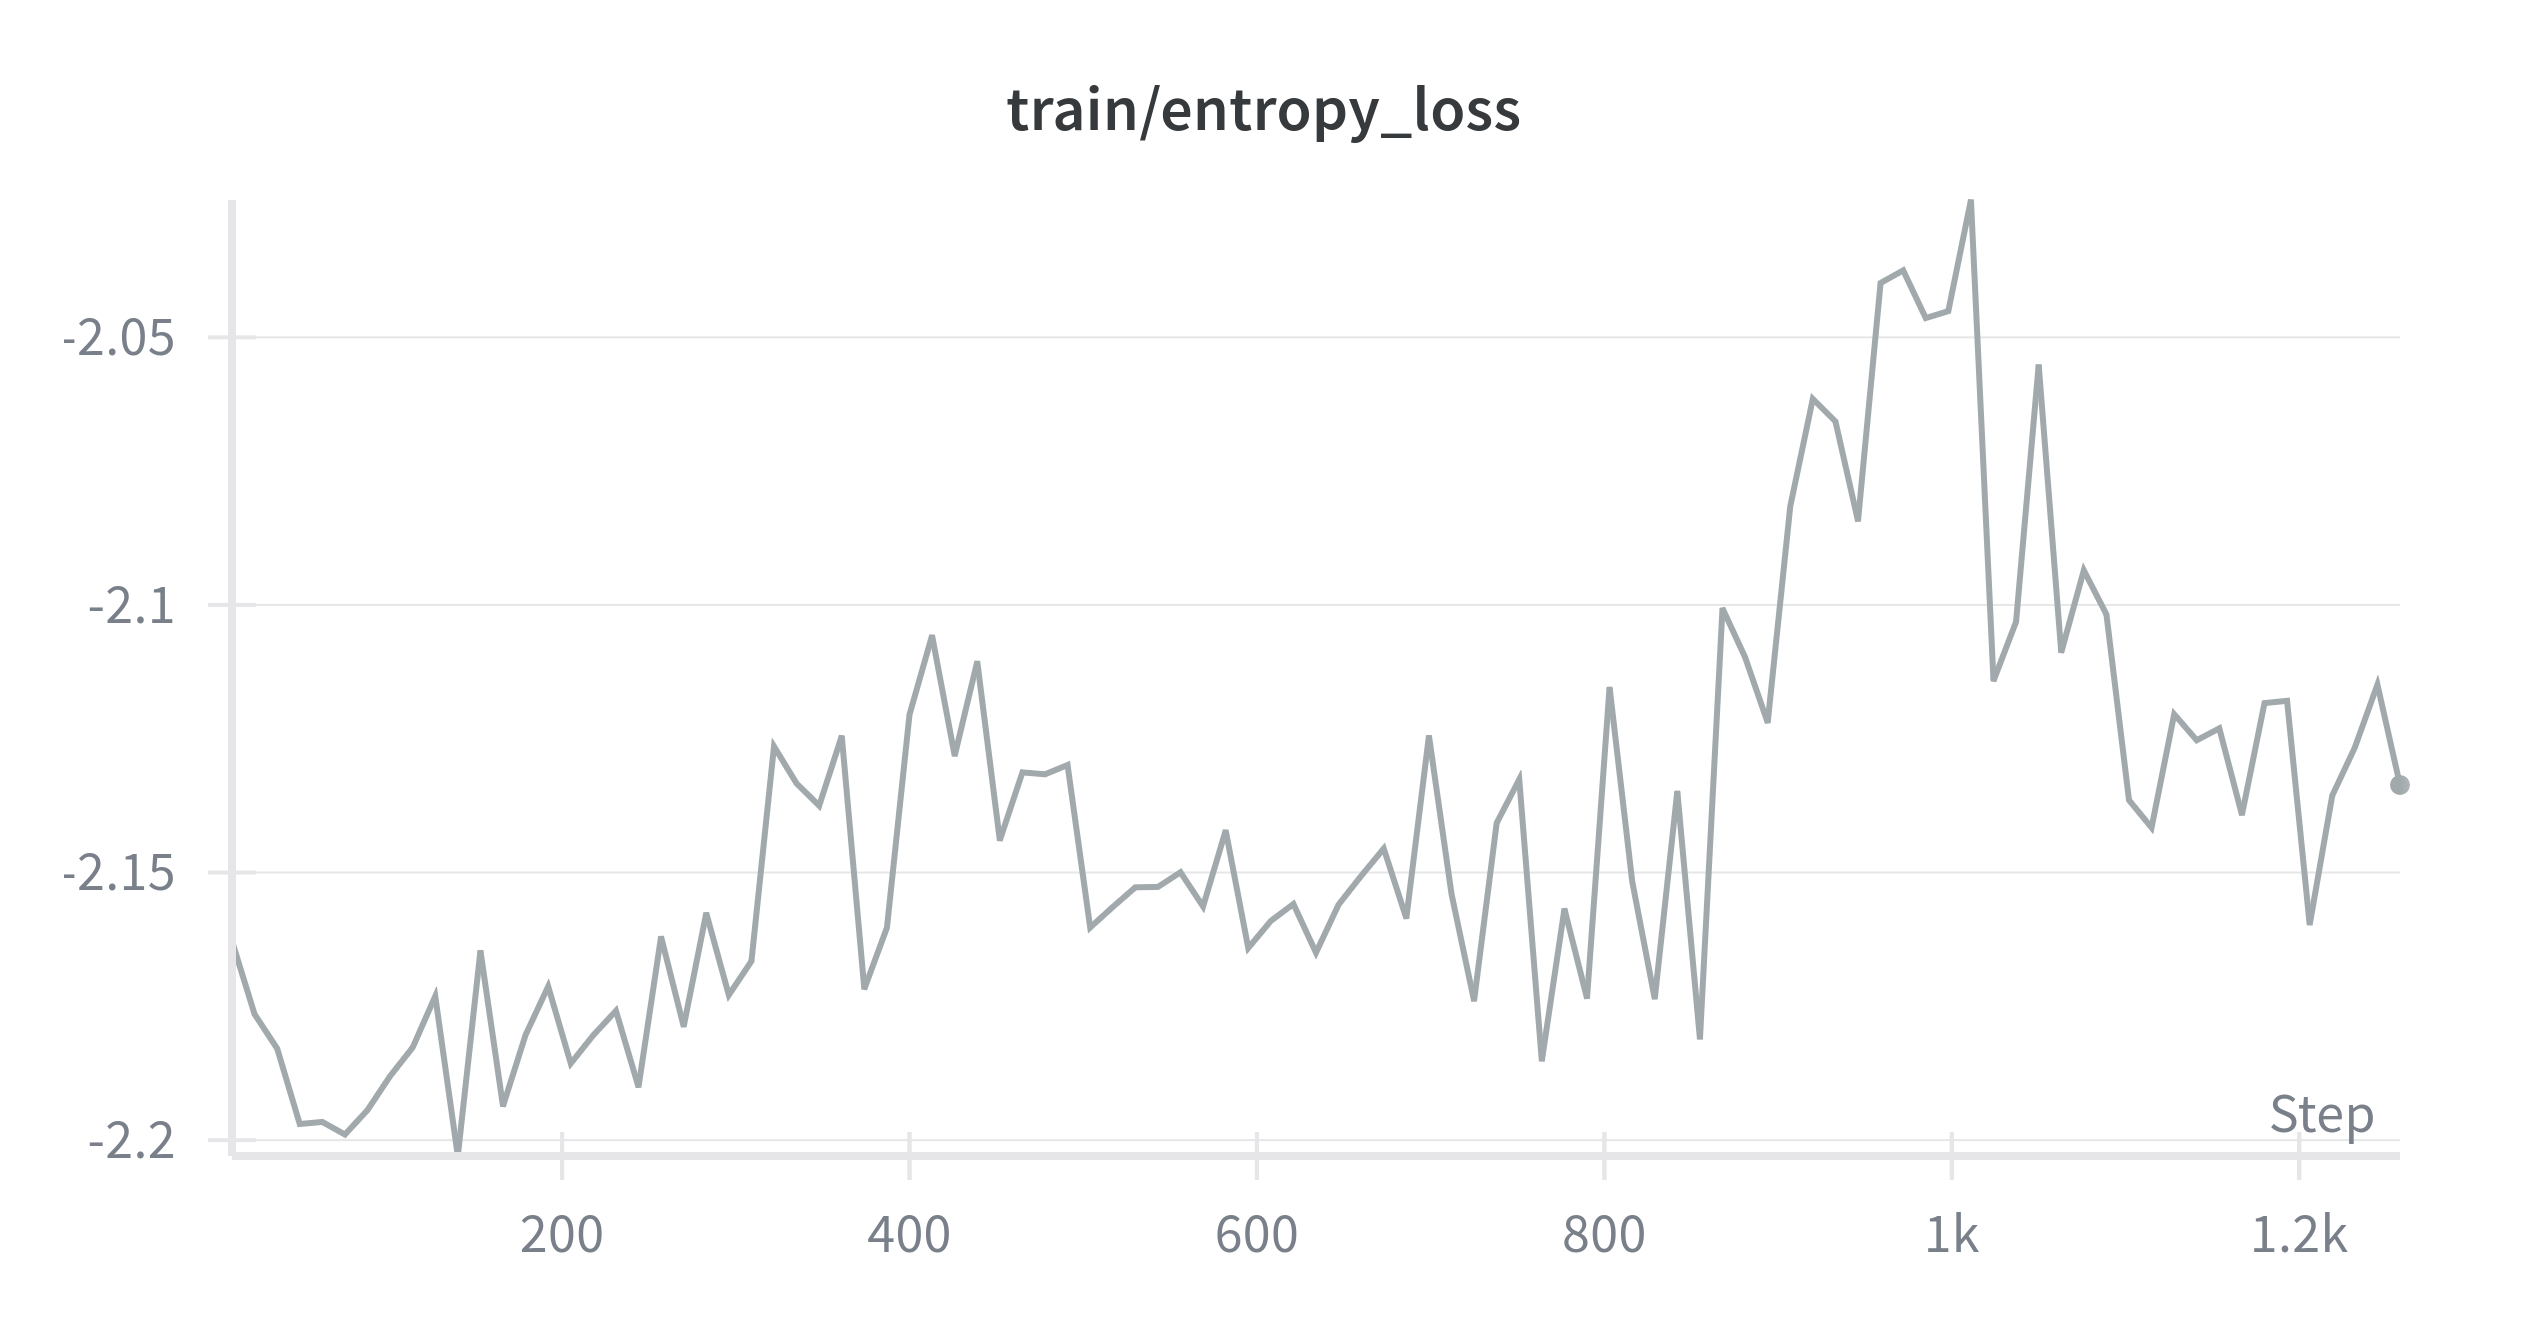
\includegraphics[width=\textwidth]{images/Entrophy Loss.png}
        \caption{Entropy loss}
        \label{fig:entropy_loss}
    \end{subfigure}\hfill
    \begin{subfigure}[t]{0.48\textwidth}
        \centering
        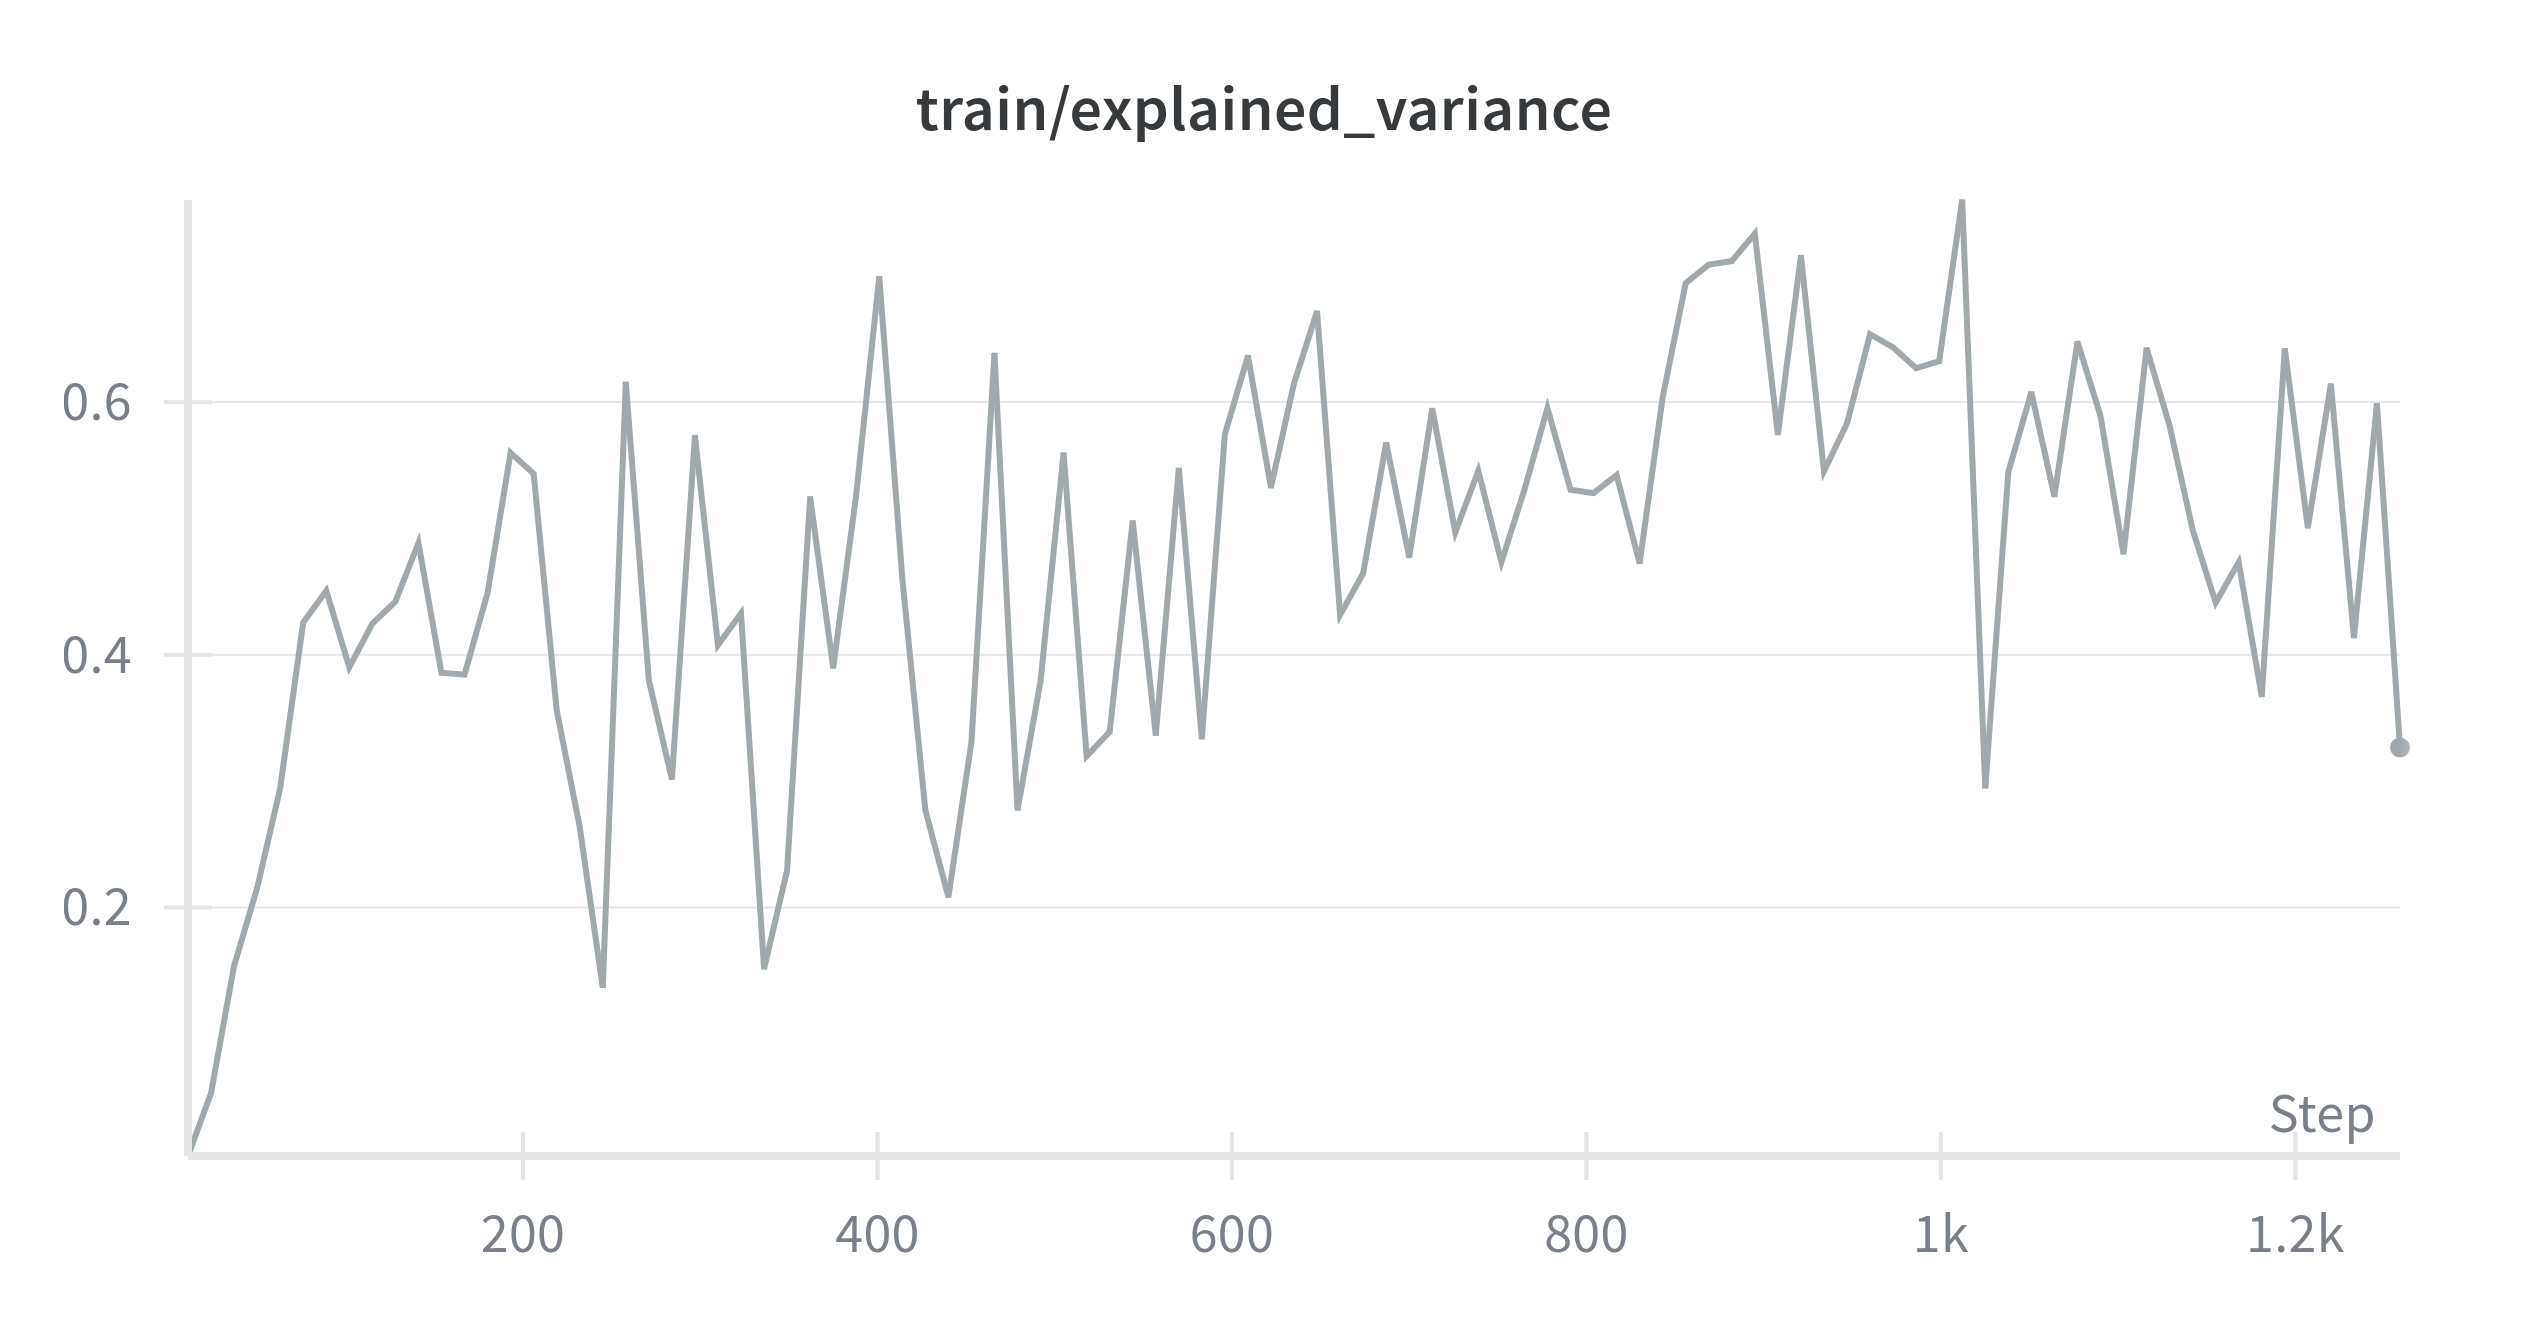
\includegraphics[width=\textwidth]{images/Explained_variance.png}
        \caption{Explained variance}
        \label{fig:explained_variance}
    \end{subfigure}

    \caption{Training curves for PPO: reward, mean match length, entropy loss, and explained variance.}
    \label{fig:ppo_training_curves}
\end{figure}

The figure \ref{fig:ppo_training_curves} shows the training curves for the PPO algorithm, including reward evolution, mean match length, entropy loss, and explained variance. The reward evolution curve indicates a steady increase in performance over time, suggesting that the agent is learning effective strategies to win matches at each stages of the curriculum learning. The mean match length curve shows a decrease in match duration, indicating that the agent is becoming more efficient at defeating opponents. The entropy loss curve demonstrates a reduction in exploration as the agent converges towards optimal policies with some difficulty which may implies that the variance of enemy should also increase. Finally, the explained variance curve reflects the accuracy of the value function approximation.

Given these metrics and the observed win rate against baseline models, we conclude that the proposed agent architecture and training procedure are effective for learning competitive strategies in the tank battle environment. But there is still room for improvement, especially in terms of exploration and adaptation to diverse opponent strategies, probably solvable by either increasing the complexity of the agent or providing more and different enemy models to the models pool.

Additionally, we provide a visual evaluation of the trained agent after 100000 timesteps in the following video: \href{https://youtu.be/GO1fE_dqkJs}{Video}.

\section{Previous approaches}

Before archiving the presenting results we had several different approaches to the agent architecture and training loop, which are described below. All of them were discarded in favor of the current approach due to their poor performance or high computational cost.

\subsection{Centralized agent}

We start the project having 3 different tanks at the same time with more internal walls (check Figure \ref{fig:initial_walls}), and fixed spawnzones for each team with a centralized agent that controlled both tanks at the same time. The observation space was the same as the current one, but the action space was different, as the agent had to output actions for both tanks at the same time. The exploration during the training process was very poor. The entropy loss basically stuck in 8.76 for the whole training process, which meant that the agent was not able to explore the environment properly.

\begin{figure}
    \centering
    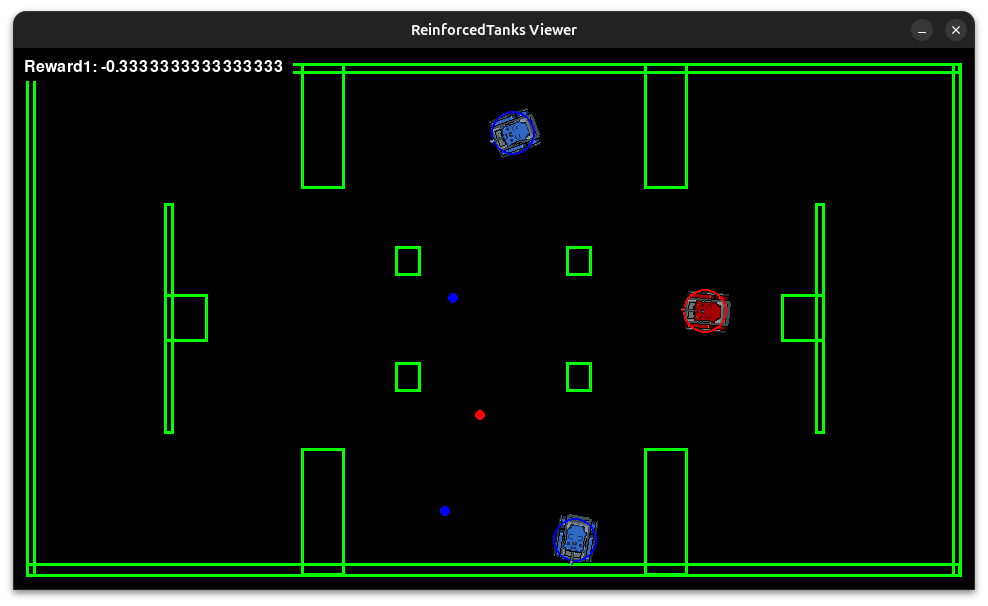
\includegraphics[width=0.5\textwidth]{images/Initial walls.png}
    \caption{Centralized agent architecture}
    \label{fig:initial_walls}
\end{figure}

\section*{Acknowledgments}

We thanks to Asier Gonzalez, who helped us realising that out first approach treating the team as a single agent was flawed.

\bibliography{sample}

\end{document}
